%!Mode:: "TeX:UTF-8"

\section{进程}

\subsection{进程与线程}
进程的四大特征:\textbf{动态性,并发性,独立性,异步性}。

进程与程序的关系:一个进程可以依次执行多个程序,多个进程可共同执行一个程序。

进程与线程的区别:
从内核的观点看,进程的目的就是担当分配系统资源(CPU时间、内存等)的基本单位。线程是进程的一个执行流,是CPU调度和分派的基本单位,它是比进程更小的能独立运行的基本单位。

进程是独立的,这表现在内存空间、上下文环境上;线程运行在进程空间内。一般来讲(不使用特殊技术),进程无法突破进程边界存取其他进程的存储空间;
而线程由于处于进程空间内,所有同一进程的线程共享同一内存空间。

线程是属于进程的,当进程退出时该进程所产生的线程都会被强制退出并清除。线程所占用的资源要少于进程所占用的资源。进程和线程都可以有优先级。

\textbf{多进程和多线程各有什么优缺点}?
进程优点:编程、调试简单,可靠性较高,适合多机、多核系统。\\
线程优点:创建、销毁、切换速度快,内存、资源占用小,数据共享简单,只适合多核系统。

\subsection{进程内存布局}
图\ref{fig:processmemlayout}为典型的内存布局(选择《APUE》)。
\begin{figure}[ht]
	\begin{center}
		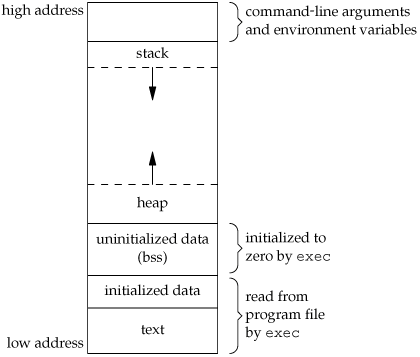
\includegraphics[keepaspectratio,width=0.5\paperwidth]{Pictures/Kernel/programMemLayout.png}
	\caption{进程的典型内存布局示例}
	\label{fig:processmemlayout}
	\end{center}
\end{figure}

《CSAPP》给出的内存布局如图\ref{fig:processmemlayout-csapp}所示。
\begin{figure}[ht]
	\begin{center}
		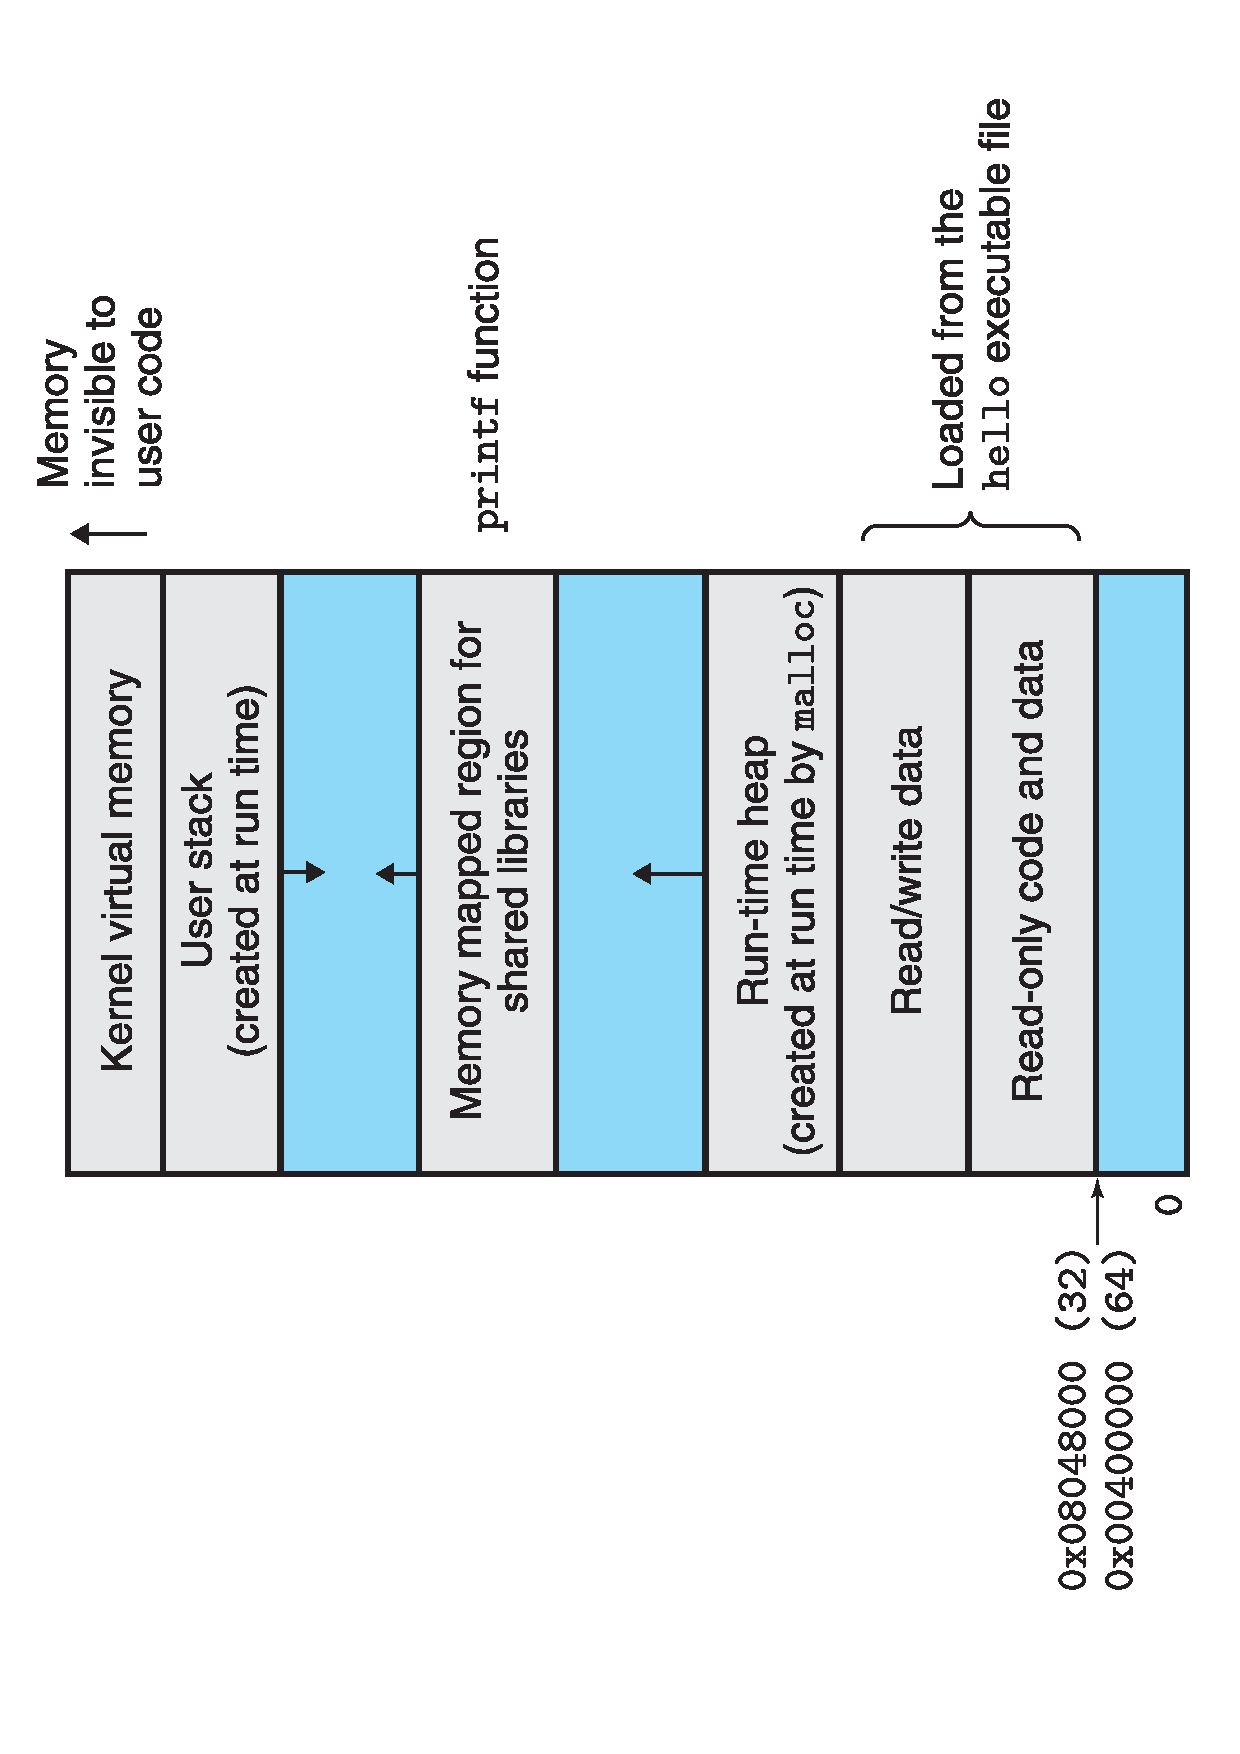
\includegraphics[keepaspectratio,width=0.5\paperwidth,angle=270]{Pictures/Kernel/process-mem-csapp.pdf}
	\caption{进程的典型内存布局示例}
	\label{fig:processmemlayout-csapp}
	\end{center}
\end{figure}

图 \ref{fig:processmemlayout-csdn}是从CSDN上找到的:
\begin{figure}[ht]
	\begin{center}
		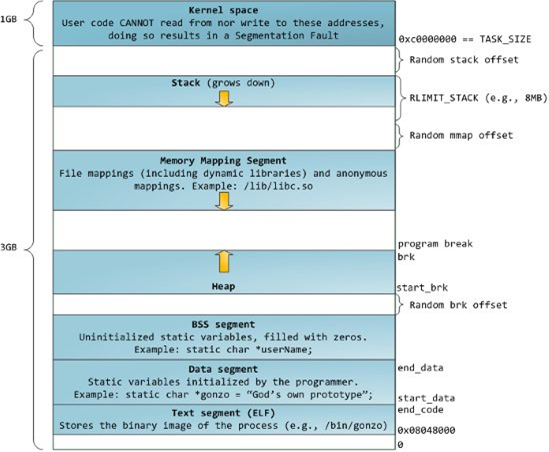
\includegraphics[keepaspectratio,width=0.5\paperwidth]{Pictures/Kernel/LinuxCppMemLayout3.png}
	\caption{进程的典型内存布局示例}
	\label{fig:processmemlayout-csdn}
	\end{center}
\end{figure}


最高地址区域又叫内核虚拟存储器,是用户代码不可见区域。
ESP指向栈顶,通过brk/sbrk系统调用扩大堆,向上增长。
小于0x0804 8000为保留区域,进而是只读段。
在glibc实现的内存管理算法中,Malloc小块内存是在小于0x4000 0000的内存中分配的,通过brk/sbrk不断向上扩展,而分配大块内存,malloc直接通过系统调用mmap实现,分配得到的地址在文件映射区,所以其地址大于0x4000 0000。
值得注意的是,字符串字面值(如"Hello World")存储在代码段(只读段)。

图\ref{fig:processmemlayout-csapp}所描述的模型无法适用于多线程环境。
按图\ref{fig:processmemlayout-csapp}所述,程序最多拥有上GB的栈空间,事实上,在多线程情况下,能用的栈空间是非常有限的, 可能只有几MB,超这个范围就会造成栈溢出。
线程的堆栈一般都是在线程创建的时候就固定分配好了的,线程切换的时候需要保存的是栈顶指针。
Windows线程的缺省堆栈大小为1M,Linux默认8M。

同一个进程中的多个线程,它们的内存空间是共享的(栈除外),在一个线程修改的内存内容,对所有线程都生效。这是一个优点也是一个缺点。说它是优点,线程的数据交换变得非常快捷。说它是缺点,一个线程死掉了,其它线程也性命不保; 多个线程访问共享数据,需要昂贵的同步开销,也容易造成同步相关的BUG。

线程间共享:地址空间,全局变量,打开文件,子进程,即将发生的报警,信号与信号处理程序,账户信息。线程私有:\textbf{程序计数器,寄存器,堆栈,状态}。
和传统进程一样(即只有一个线程的进程),线程可以处于若干种状态的任何一个:运行、阻塞、就绪或终止。 
线程自己的堆栈往往属于进程堆栈的一部分,thread switch时通常无需专门进行保存。thread switch时,往往只需要保存寄存器信息,故switch的开销较小。

\subsection{Linux进程结构}
files\_struct结构保存了进程打开的所有文件表数据,描述一个正被打开的文件。

struct file文件结构体代表一个打开的文件,系统中的每个打开的文件在内核空间都有一个关联的struct file。它由内核在打开文件时创建,并传递给在文件上进行操作的任何函数。在文件的所有实例都关闭后,内核释放这个数据结构。在内核创建和驱动源码中,struct file的指针通常被命名为file或filp。struct file包含的struct file\_operations成员包含着与文件关联的操作,如seek,read,write。

\begin{figure}[ht]
	\begin{center}
		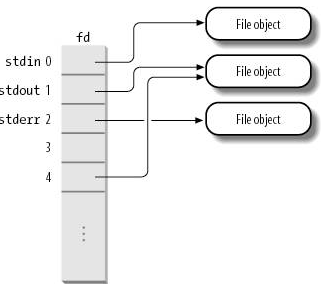
\includegraphics[keepaspectratio,width=0.3\paperwidth]{Pictures/Kernel/LinuxFdArrayInFileStruct.png}
	\caption{file\_struct中的fd数组}
	\label{fig:LinuxFdArrayInFileStruct}
	\end{center}
\end{figure}

\begin{figure}[ht]
	\begin{center}
		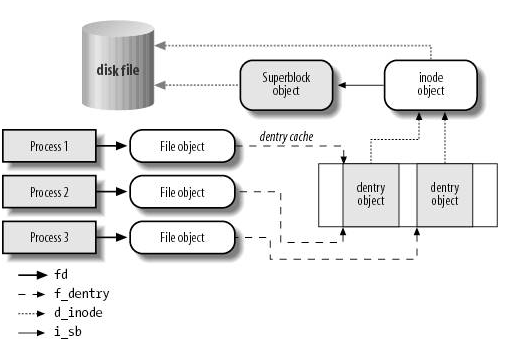
\includegraphics[keepaspectratio,width=0.4\paperwidth]{Pictures/Kernel/LinuxProcessAndVFS.png}
	\caption{进程与VFS的交互}
	\label{fig:LinuxProcessAndVFS}
	\end{center}
\end{figure}

\subsection{Linux线程模型}

线程的实现分为两种方式,多对一模型和一对一模型。
多对一模型下,内核对线程无知,以进程为调度单位,而线程调度是由用户进程完成的,可理解成进程将内核分配给自己的时间片二次分配给自己的线程。
此设计缺点明显:线程的阻塞导致进程阻塞。
一对一模型下,内核以线程为单位进行调度,LinuxThreads和NPTL均使用一对一模型。

LinuxThread使用clone系统调用来产生“线程”,这里的线程虽符合轻量进程的定义, 但它又具备了进程的若干特性,如拥有独立的进程id和信号机制等等。
内核在进行调度时,仍然按照传统的进程调度机制,在这个意义上,是将“线程”当作进程来处理的,内核对线程并无特殊支持。

 LinuxThreads 设计的一些局限性:
 \begin{itemize}
 \item 由于它是围绕一个管理线程来设计的,因此会导致很多的上下文切换的开销,这可能会妨碍系统的可伸缩性和性能。
 由于管理线程只能在一个 CPU 上运行,因此所执行的同步操作在 SMP 或 NUMA 系统上可能会产生可伸缩性的问题。
 \item 由于线程的管理方式,以及每个线程都使用了一个不同的进程 ID,对信号的处理是按照每线程的原则建立的, 因此 LinuxThreads 与其他与 POSIX 相关的线程库并不兼容。
 \item 由于内核实际上将线程“认作”进程,因此针对进程的诸多限制也被应用在线程上,比如可用进程总数等, /proc下也有大量进程项对应线程。
 \end{itemize}

NPTL,或称为 Native POSIX Thread Library,是 Linux 线程的一个新实现,它克服了 LinuxThreads 的缺点,同时也符合 POSIX 的需求。
与 LinuxThreads 相比,它在性能和稳定性方面都提供了重大的改进。自2.6内核以来,NPTL取代LinuxThreads成为了新的Linux线程标准。

NPTL使用了跟LinuxThread相同的办法,在内核里面线程仍然被当作是一个进程,并且仍然使用了clone()系统调用(在NPTL库里调用)。
但是,NPTL需要内核级的特殊支持来实现,比如需要挂起然后再唤醒线程的线程同步原语futex。

与 LinuxThreads 相比,NPTL 具有很多优点: NPTL没有使用管理线程。
管理线程的一些需求,例如向作为进程一部分的所有线程发送终止信号,是并不需要的;因为内核本身就可以实现这些功能。
内核还会处理每个线程堆栈所使用的内存的回收工作。它甚至还通过在清除父线程之前进行等待,从而实现对所有线程结束的管理,这样可以避免僵尸进程的问题。
由于 NPTL 没有使用管理线程,因此其线程模型在 NUMA 和 SMP 系统上具有更好的可伸缩性和同步机制。

\subsection{Thread-local storage}
Thread-local storage (TLS) 指“局部”于线程的静态/全局地址位置,实际上是说当多个线程引用同一静态/全局变量时,实际上是引用了不同的地址位置。

Windows API和Pthread均提供了操纵TLS变量的接口。C++11 引人了thread\_local 关键词,定义TLS变量,此外,gcc使用如\verb$__thread int number;$语法定义TLS。
Python如此使用TLS:

\begin{lstlisting}[language=Python]
import threading
mydata = threading.local()
mydata.x = 1
\end{lstlisting}

\subsection{进程同步}
进程同步是一个操作系统级别的概念,是在多道程序的环境下,存在着不同的制约关系,为了协调这种互相制约的关系,实现资源共享和进程协作,从而避免进程之间的冲突,引入了进程同步。

进程同步的机制有:
\begin{itemize}
\item 信号量
\item 自旋锁
\item 原子操作
\item 管程
\item 会和
\item 分布式系统
\end{itemize}

管程 (英语:Moniters,也称为监视器) 是一种程序结构,结构内的多个子程序(对象或模块)形成的多个工作线程互斥访问共享资源。这些共享资源一般是硬件设备或一群变量。管程实现了在一个时间点,最多只有一个线程在执行管程的某个子程序。与那些通过修改数据结构实现互斥访问的并发程序设计相比,管程实现很大程度上简化了程序设计。
管程提供了一种机制,线程可以临时放弃互斥访问,等待某些条件得到满足后,重新获得执行权恢复它的互斥访问。
东尼·霍尔证明了这与信号量是等价的。在编程语言Concurrent Pascal,Pascal-Plus,Modula-2,Modula-3,Mesa以及Java中都提供这个功能。

一个管程包含:多个彼此可以交互并共用资源的线程,多个与资源使用有关的变量,一个互斥锁,一个用来避免竞态条件的不变量。
一个管程的程序在运行一个线程前会先取得互斥锁,直到完成线程或是线程等待某个条件被满足才会放弃互斥锁。若每个执行中的线程在放弃互斥锁之前都能保证不变量成立,则所有线程皆不会导致竞态条件成立。

当一个线程执行管程中的一个子程序时,称为占用(occupy)该管程. 管程的实现确保了在一个时间点,最多只有一个线程占用了该管程。这是管程的互斥锁访问性质。

\subsection{僵尸进程}
在UNIX 系统中,一个进程结束了,但是他的父进程没有等待(调用wait/waitpid)他, 那么他将变成一个\textbf{僵尸进程}。
系统调用exit,它的作用是使进程退出,但也仅仅限于将一个正常的进程变成一个僵尸进程,并不能将其完全销毁。
即使是root身份kill-9也不能杀死僵尸进程。
补救办法是杀死僵尸进程的父进程(僵尸进程的父进程必然存在),僵尸进程成为"孤儿进程",过继给1号进程init,init始终会负责清理僵尸进程。
在Linux进程的状态中,僵尸进程是非常特殊的一种,它已经放弃了几乎所有内存空间,没有任何可执行代码,也不能被调度,仅仅在进程列表中保留一个位置,
记载该进程的退出状态等信息供其他进程收集,除此之外,僵尸进程不再占有任何内存空间。
僵尸进程占用了进程号资源,同时记录着进程的退出状态、进程运行的CPU时间等。

为避免僵尸进程,父进程可以用signal函数为SIGCHLD安装handler,因为子进程结束后, 父进程会收到该信号,可以在handler中调用wait回收;
也可以用signal(SIGCHLD,SIG\_IGN) 通知内核,自己对子进程的结束不感兴趣,那么子进程结束后,内核会回收,并不再给父进程发送信号。

\subsection{进程通信}
共享存储系统、消息传递系统、管道(以文件系统为基础)。

信号的处理方式包括:忽略,捕捉(调用用户函数),执行默认动作。
有两种信号不能忽略:SIGKILL,SIGSTOP。它们向超级用户提供了使进程终止或停止的可靠方法。

\subsection{协程与线程的区别}
1. 协程并非os线程,所以创建、切换开销比线程相对要小。
        2. 协程与线程一样有自己的栈、局部变量等,但是协程的栈是在用户进程空间模拟的,所以创建、切换开销很小。
        3. 多线程程序是多个线程并发执行,也就是说在一瞬间有多个控制流在执行。而协程强调的是一种多个协程间协作的关系,只有当一个协程主动放弃执行权,另一个协程才能获得执行权,所以在某一瞬间,多个协程间只有一个在运行。
        4. 由于多个协程时只有一个在运行,所以对于临界区的访问不需要加锁,而多线程的情况则必须加锁。
        5. 多线程程序由于有多个控制流,所以程序的行为不可控,而多个协程的执行是由开发者定义的所以是可控的。


\clearpage
















